\documentclass[tikz,border=12pt]{standalone}
% Match the sans-serif font stack used by the Minimal Mistakes site theme.
% TeX Gyre Heros is the TeX-compatible Helvetica implementation.
\usepackage[T1]{fontenc}
\usepackage{tgheros}
\renewcommand{\familydefault}{\sfdefault}

\usepackage{amsmath}
\usetikzlibrary{arrows.meta,positioning}

\definecolor{bluefill}{HTML}{E7F5FF}
\definecolor{blueedge}{HTML}{1971C2}
\definecolor{greenfill}{HTML}{EBFBEE}
\definecolor{greenedge}{HTML}{2B8A3E}
\definecolor{ink}{HTML}{343A40}

\begin{document}
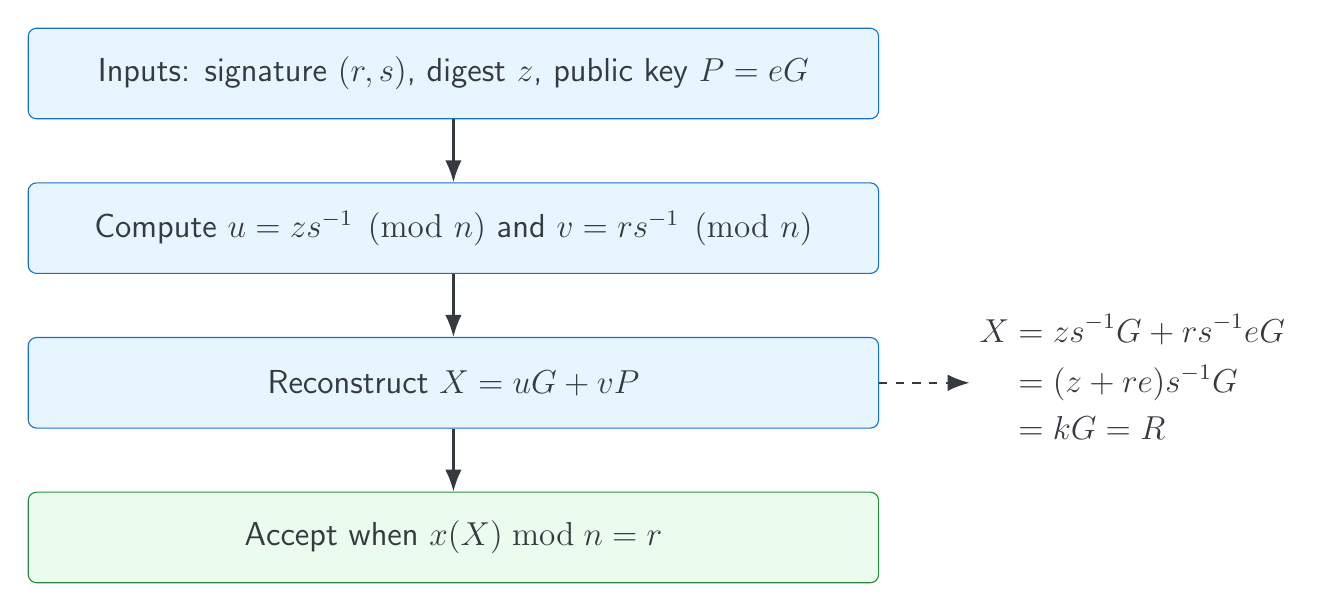
\begin{tikzpicture}[
  node distance=0.8cm,
  box/.style={draw=blueedge, fill=bluefill, rounded corners=3pt, minimum width=10.8cm,
    minimum height=1.15cm, align=center, font=\large, text=ink},
  result/.style={draw=greenedge, fill=greenfill, rounded corners=3pt, minimum width=10.8cm,
    minimum height=1.15cm, align=center, font=\large, text=ink},
  arrow/.style={-{Latex[length=2.8mm]}, thick, ink}
]
  \node[box] (inputs) {Inputs: signature $(r,s)$, digest $z$, public key $P=eG$};
  \node[box, below=of inputs] (scalars) {Compute $u=zs^{-1}\pmod n$ and $v=rs^{-1}\pmod n$};
  \node[box, below=of scalars] (point) {Reconstruct $X=uG+vP$};
  \node[result, below=of point] (check) {Accept when $x(X)\bmod n=r$};

  \draw[arrow] (inputs) -- (scalars);
  \draw[arrow] (scalars) -- (point);
  \draw[arrow] (point) -- (check);

  \node[anchor=west, align=left, font=\large, text=ink, right=1.15cm of point] (proof) {$\begin{aligned}
    X &= zs^{-1}G+rs^{-1}eG\\
      &= (z+re)s^{-1}G\\
      &= kG=R
  \end{aligned}$};
  \draw[arrow, dashed] (point.east) -- (proof.west);
\end{tikzpicture}
\end{document}
